\hypertarget{atomic_8h}{}\section{/home/andressanchez/\+Escritorio/\+G\+I\+T/project\+\_\+template/src/modules/u\+O\+R\+B/include/atomic.h File Reference}
\label{atomic_8h}\index{/home/andressanchez/\+Escritorio/\+G\+I\+T/project\+\_\+template/src/modules/u\+O\+R\+B/include/atomic.\+h@{/home/andressanchez/\+Escritorio/\+G\+I\+T/project\+\_\+template/src/modules/u\+O\+R\+B/include/atomic.\+h}}
This graph shows which files directly or indirectly include this file\+:\nopagebreak
\begin{figure}[H]
\begin{center}
\leavevmode
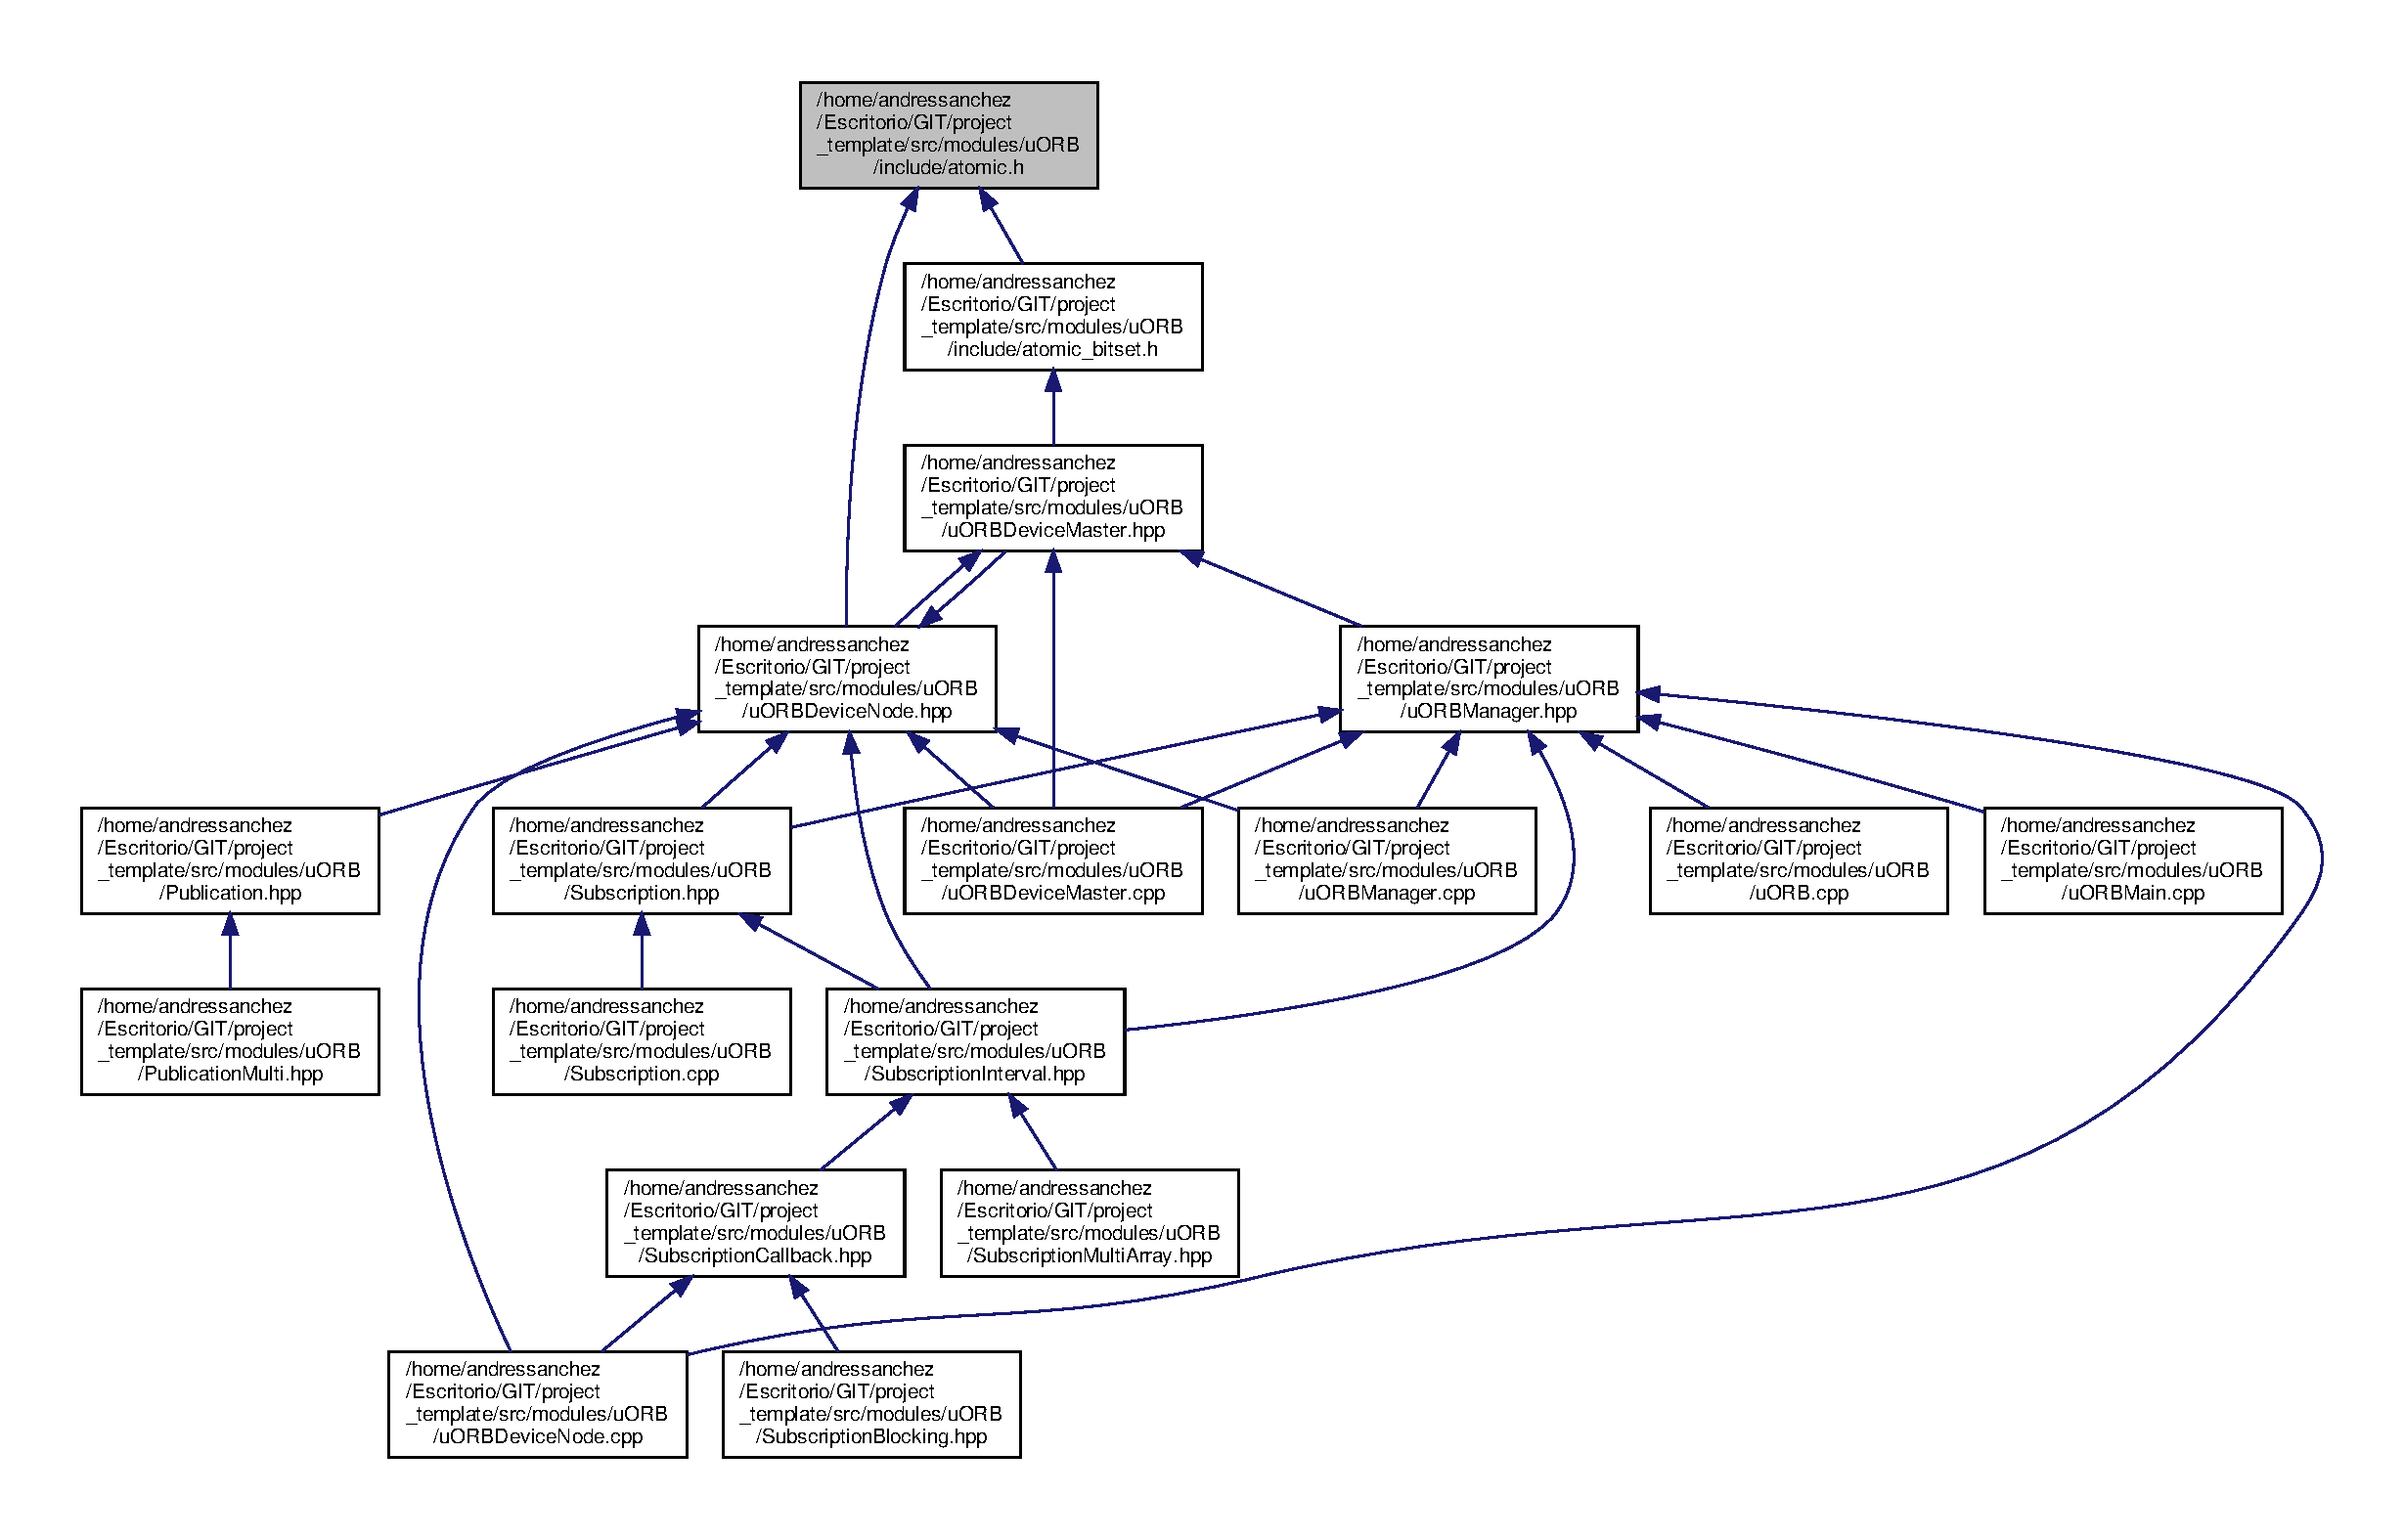
\includegraphics[width=350pt]{d6/d08/atomic_8h__dep__incl}
\end{center}
\end{figure}


\subsection{Detailed Description}
Provides atomic integers and counters. Each method is executed atomically and thus can be used to prevent data races and add memory synchronization between threads.

In addition to the atomicity, each method serves as a memory barrier (sequential consistent ordering). This means all operations that happen before and could potentially have visible side-\/effects in other threads will happen before the method is executed.

The implementation uses the built-\/in methods from G\+CC (supported by Clang as well). \begin{DoxySeeAlso}{See also}
\href{https://gcc.gnu.org/onlinedocs/gcc/_005f_005fatomic-Builtins.html}{\tt https\+://gcc.\+gnu.\+org/onlinedocs/gcc/\+\_\+005f\+\_\+005fatomic-\/\+Builtins.\+html}.
\end{DoxySeeAlso}
\begin{DoxyNote}{Note}
\+: on A\+RM, the instructions L\+D\+R\+EX and S\+T\+R\+EX might be emitted. To ensure correct behavior, the exclusive monitor needs to be cleared on a task switch (via C\+L\+R\+EX). This happens automatically e.\+g. on A\+R\+Mv7-\/M as part of an exception entry or exit sequence. 
\end{DoxyNote}
